%-----------------------------------------------
%   LaTeX template
%   Crée par: Thorkel-dev
%-----------------------------------------------

\documentclass[a4paper,11pt,titlepage]{article}

\usepackage{lipsum}

\usepackage[
            imageFooterLeft      =  {latex.png},                        % Optionnel
            imageHeaderLeft      =  {eseo.png},                         % Optionnel
            %subject              =  {{Subject of the document}},        % Optionnel
            %keywords             =  {{Example, Template, LaTeX}},       % Optionnel
            language             =  {french},                      
            % encoding             =  {},                               % Defaut utf8
            ]{Parameter}

\usepackage[
            logoRight       =   {ST-logo.png},                          % Optionnel
            logoLeft        =   {eseo.png},                             % Optionnel
            %logoCenter      =   {latex.png},                          % Optionnel
            subject         =   {{Incrément 2}},                        % Optionnel
            projectName     =   {PSC~(Prototype~Sonnette~Connectée)},    % Optionnel
            enterpriseName  =   {STMicroelectronics},                   % Optionnel
            responsableName =   {Hugo~BOUY},                            % Optionnel
            etatDocument    =   {Version~finale},                       % Optionnel
            %revision        =   {},                                   % Optionnel
            version         =   {2.5},                                  % Optionnel
            ]{FrontPage}

\makeglossaries
\loadglsentries{glossary.tex} % Charge le glossaire
\loadglsentries{acronyms.tex} % Charge les acronymes
\addbibresource{biblio.bib}   % Charge la bibliographie

%-----------------------------------------
%      Variables
%-----------------------------------------
\author{ProSE~2024~A1}        % Auteur
\title{Dossier de spécification}     % Titre
\date{\normalsize\today}    % Date actuelle, automatique
\newcommand{\client}{STMicroelectronics}
\newcommand{\groupe}{Prose-2024-A1}
\newcommand{\equipe}{Projet Prose A1}

\graphicspath{{../schemas/}{../figures/}}


%Hyphenation
%\hyphenation{STMicroelectronics}


% Exemple d'arrière plan
\backgroundsetup{
    scale=1,
    opacity=0.1,
    angle=0,
    contents={%
            \includegraphics[width=\textwidth]{eseo.png}
        }%
}

\setlength{\parskip}{0.5em} % Espacement entre les paragraphes
\setlength{\belowcaptionskip}{-0.5em} % Espacement entre les images
%\setlength{\parindent}{0pt} % Pas d'indentation
\setcounter{tocdepth}{3}

%-----------------------------------------
%      Document
%-----------------------------------------

\begin{document}

\maketitle

\BgThispage % Utiliser l'arrière plan
\vspace*{\fill}
\noindent
AVERTISSEMENT : \\
Le présent document est un document à but pédagogique.
Il a été réalisé sous la direction de Jérôme DELATOUR, en collaboration avec des enseignants et les étudiants de l'option SE, groupe A1 (Hugo BOUY, Bastien CASSAR, Paul CHIRON, Paul JURET, Laurent LETENNEUR, Mathis MOULIN, Romain TROVALLET) du groupe ESEO.
Ce document est la propriété de Jérôme DELATOUR du groupe ESEO. En dehors des activités pédagogiques de l'ESEO, ce document ne peut être diffusé ou recopié sans l'autorisation écrite de ses propriétaires.
\vspace*{\fill}
\clearpage

\section*{Table des versions}
\begin{xltabular}{\linewidth}{|c|X|>{\centering\arraybackslash}X|c|c|}

    \hline \textbf{Date} & \textbf{Actions} & \textbf{Auteur} & \textbf{Version} & \textbf{Révision} \\\hline
    \endfirsthead

    \multicolumn{5}{l}%
    {\textbf{}}\\
    \hline \textbf{Date} & \textbf{Actions} & \textbf{Auteur} & \textbf{Version} & \textbf{Révision} \\\hline
    \endhead

    \multicolumn{5}{r}%
    {\textbf{}}\tabularnewline
    \endfoot
    \endlastfoot
    27/05/2023 & Divers corrections de typos et de cohérence & Romain TROVALLET & 2.5 & 0 \\ \hline
    27/05/2023 & Correction divers (typo, cohérence) & Hugo BOUY & 2.4 & 0 \\ \hline
    27/05/2023 & Ajout de la Pop-up et de la logique vidéo indisponible et suppression de TAM & Hugo BOUY & 2.3 & 1 \\ \hline
    27/05/2023 & Suppression du moteur & Hugo BOUY & 2.3 & 0 \\ \hline
    25/05/2023 & Relecture et correction diverse après AN & Hugo BOUY et Romain TROVALLET & 2.2 & 0 \\ \hline
    25/05/2023 & Correction des CU et des fonctions après AN & Hugo BOUY & 2.1 & 1 \\ \hline
    24/05/2023 & Ajout descriptions manquantes dans contexte physique & Hugo BOUY & 2.1 & 0 \\ \hline
    23/05/2023 & Relecture et validation pour AN Spec du 24/05/2023 & Toute l'équipe & 2.0 & 0 \\ \hline
    22/05/2023 & Suppression du terme "Base de données" & Hugo BOUY & 1.5 & 1 \\ \hline
    22/05/2023 & Mise à jour du CU Ouvrir Porte & Hugo BOUY & 1.5 & 0 \\ \hline
    22/05/2023 & Mise à jour des CU avec la communication entre AOP et SS & Hugo BOUY & 1.4 & 1 \\ \hline
    22/05/2023 & Mise à jour du CU Initialiser Board & Hugo BOUY & 1.4 & 0 \\ \hline
    22/05/2023 & Mise à jour CU Consulter Calendrier + CU Reconnaître Visage & Romain TROVALLET & 1.3 & 0 \\ \hline
    09/05/2023 & Correction avant Incrément 2 & Romain TROVALLET & 1.2 & 0 \\ \hline
    21/03/2023 & Correction des CUs après AC & Laurent LETENNEUR & 1.1 & 3 \\ \hline
    20/03/2023 & Correction architecture matérielle après AC & Hugo BOUY & 1.1 & 2 \\ \hline
    18/03/2023 & Màj des références documentaires & Paul CHIRON & 1.1 & 1 \\ \hline
    17/03/2023 & Corrections mineurs en live de l'AC Spec & Paul JURET et Romain TROVALLET & 1.1 & 0 \\ \hline
    16/03/2023 & Relecture et validation pour AC Spec du 17/03/2023 & Toute l'équipe & 1.0 & 0 \\ \hline
    15/03/2023 & Màj archi matérielle et description générale après consulting & Hugo BOUY & 0.9 & 1 \\ \hline
    15/03/2023 & Ajout des parties 2.4, 2.5 et 2.6 & Paul JURET & 0.9 & 0 \\ \hline
    15/03/2023 & Modification des CUs & Laurent LETENNEUR & 0.8 & 7 \\ \hline
    15/03/2023 & Relecture CUs & Paul CHIRON & 0.8 & 6 \\ \hline
    15/03/2023 & Modification contexte physique & Paul JURET & 0.8 & 5 \\ \hline
    15/03/2023 & Ajout de mots aux dictionnaire du domaine et des hyperliens & Bastien CASSAR & 0.8 & 4 \\ \hline
    13/03/2023 & Correction des CUs, mise en page et dictionnaire de domaine & Hugo BOUY & 0.8 & 3 \\ \hline
    12/03/2023 & Modification des CUs & Laurent LETENNEUR & 0.8 & 2 \\ \hline
    12/03/2023 & Modification bibliographie et dictionnaire de domaine & Paul CHIRON & 0.8 & 1 \\ \hline
    12/03/2023 & Modifications et finitions contexte physique & Mathis MOULIN & 0.8 & 0 \\ \hline
    12/03/2023 & Relecture des CUs & Paul CHIRON & 0.7 & 1 \\ \hline
    11/03/2023 & Ajout des CUs & Laurent LETENNEUR & 0.7 & 0 \\ \hline
    10/03/2023 & Relecture description générale et caractéristiques des acteurs & Hugo BOUY & 0.6 & 1 \\ \hline
    09/03/2023 & Modifications et finitions contexte logique & Bastien CASSAR & 0.6 & 0 \\ \hline
    08/03/2023 & Modification Intro et Acteurs & Paul CHIRON & 0.5 & 1 \\ \hline
    08/03/2023 & Ajout partie description générale & Paul JURET & 0.5 & 0 \\ \hline
    08/03/2023 & Modification IHM et Modification MàE & Bastien CASSAR & 0.4 & 2 \\ \hline
    07/03/2023 & Modification acronymes et dictionnaire de domaine & Paul CHIRON & 0.4 & 1 \\ \hline
    07/03/2023 & Ajout partie architecture matérielle & Hugo BOUY & 0.4 & 0 \\ \hline
    06/03/2023 & Ajout des descriptions générale et textuelles & Mathis MOULIN & 0.3 & 2 \\ \hline
    06/03/2023 & Ajout d'une IHM & Bastien CASSAR & 0.3 & 1 \\ \hline
    05/03/2023 & Ajout partie Acteurs & Paul CHIRON & 0.3 & 0 \\ \hline
    05/03/2023 & Ajout partie Intro & Paul CHIRON & 0.2 & 0 \\ \hline
    04/03/2023 & Ajout partie IHM et Modification MàE & Bastien CASSAR & 0.1 & 0 \\ \hline
    02/03/2023 & Création du document & Paul CHIRON & 0.0 & 0 \\ \hline
    
\end{xltabular}
 \label{TableOfVersion} % Ajoute la table des versions
\clearpage

\addtocontents{toc}{\protect\setlength{\parskip}{0pt}}
\tableofcontents % Ajoute la table des matières

%-----------------------------------------
%      Partie I
%-----------------------------------------

\section{Introduction}

\subsection{Objet}

Ce dossier de conception a pour objectif de rassembler toute la conception du logiciel PSC. 
Il permettra à l’équipe A1 de développer le logiciel ainsi qu’élaborer des tests.

Les éléments de conception présentés dans ce document ont été déterminés suite à l’étude du dossier de spécification \refSpec.

Ce dossier de conception suit les recommandations de la norme IEEE 29148 [IEEE-29148:2018]. 
Il utilise des schémas et illustrations respectant la norme UML en version 2.5.1 [UML\_2.5.1\_2017].
Il respecte les exigences du Plan d’Assurance Qualité Logicielle (PAQL) défini par l’équipe A1 \refPAQL.


\subsection{Portée}

Ce document décrit les éléments de conception du Système à l'Étude (SàE). Il est destiné :

\begin{itemize}
    \item À l'équipe de développement C et celle de développement Android afin de préciser l'implémentation des objets constituant le SàE.
    \item Aux testeurs, afin qu'ils puissent élaborer les tests adéquats vérifiant la philosophie de conception adaptée par l'équipe.
    \item Aux auditeurs de la société FORMATO lors de leurs différents suivis du projet.
    \item Au client pour que le cadre du projet et la direction prise par l'équipe soient claires et dans la continuité des spécifications.
\end{itemize}



\newpage
\newpage
\setglossarysection{subsection}
\printglossary[type=\acronymtype,style=longborder ,title={Définitions, acronymes et abréviations}]
\glsaddallunused

\subsection{Références}

\begin{table}[H]
    \centering
    \begin{tabularx}{\textwidth}{|X|X|}
      \hline 
        \textbf{Document}  & \textbf{Référence}   \\
        \hline
        [ISO/IEC/IEEE 29148:2018]               & ISO/IEC/IEEE, “International Standard, Systems and software engineering — Life cycle processes — Requirements engineering”, version du 30/11/2018
        
        https://standards.ieee.org/standard/29148-2018.html \\ 
        \hline
        [UML\_2.5.1\_2017]                      & OMG, “Unified Modeling Language”, version 2.5.1 de décembre 2017                                                                                                                           \\ 
        \hline
        [PAQL\_A1]                             & \og Plan d'Assurance Qualité Logicielle \fg version 4.0 du 15/05/2023. 
        
        Dépôt SE 2024 A1 - ST.doc, chemin d'accès: /qualite/livrable/PAQL\_A1.pdf        \\ 
        \hline
        [ST\_Sonnette\_connectée\_industrielle\_2023] & \client, \og Cahier des charges initial pour le projet \fg, version original du 09/02/2023.
        
        Dépôt SE 2024 A1 - ST.doc, chemin d'accès: /gestion\_de\_projet/client/ ST\_Sonnette\_connectée\_industrielle.pdf               \\ 
        \hline                                  
        [CR\_R2\_09\_02\_2023]                  & \og Compte rendu de la réunion du 09/02/2023 avec les clients \fg.
        
        Dépôt SE 2024 A1 - ST.doc, chemin d'accès: /gestion\_de\_projet/réunions/ CR\_R2\_09\_02\_2023.pdf               \\ 
        \hline
    \end{tabularx}
    \caption{Références des documents utilisés dans ce dossier}
    \label{tableau-references}
  \end{table}
  

\subsection{Vue d'ensemble}
Ce document de spécification est structuré en trois parties :
\begin{itemize}
      \item La partie I définit l’objet et la portée du document ainsi qu’une liste des abréviations utilisées dans ce document et les références des documents cités.
      \item La partie II, intitulée \og description générale \fg{}, a pour objectif de présenter l'environnement et le contexte du PSC, ainsi que les fonctionnalités principales attendues pour "SoftSonnette", "SoftPorte" et "AOP".
      \item La partie III présente en détail les IHM attendues du PSC, les fonctionnalités détaillées ainsi que le dictionnaire du domaine.
\end{itemize}

Les mots en italiques sont des liens symboliques.
Certains nom d'écran des IHM sont également des liens symboliques.
Le symbole \og * \fg est un lien vers la description d'une fonction.

 % Exemple d'inclusion de fichier

%-----------------------------------------
%      Partie II
%-----------------------------------------

\newpage
\section{Description générale}

En l'absence d'un démonstrateur des capacités de sa carte STM32MP15, la société STMicroelectronics souhaite disposer d'un exemple d'application utilisant la reconnaissance faciale et divers fonctionnalités de sa carte pour les présenter à ses clients.
%La société STMicroelectronics souhaite, à terme, disposer d'un démonstrateur des capacités de sa carte, la STM32MP15. 
%Elle souhaite pouvoir présenter à ses clients un exemple d'application utilisant la reconnaissance faciale et divers fonctionnalités de la carte.

Pour ce faire, STMicroelectronics souhaite développer un prototype de sonnette connectée basé sur la reconnaissance faciale et déployé sur une STM32MP15.
Elle a donc mandaté le groupe ProSE A1 de l'ESEO afin de tester la faisabilité d'un tel prototype.

Les objectifs de ce prototype sont, premièrement, de prouver que la STM32MP15 est capable d'embarquer un programme de reconnaissance faciale et, deuxièmement, de montrer sa capacité de le faire tout en gérant l'envoi et l'affichage d'un flux vidéo. 
Ce prototype ayant pour raison d'être la démonstration des fonctionnalités de la carte STM32MP15, l'utilisation simultanée du Microprocesseur et du Microcontrôleur embarqué est attendue.
Enfin le client attend de ce prototype une interface utilisateur via une application téléphone.

%Inc
% \textbf{Le présent document spécifie l'incrément 1 du prototype.}
% Il ne traite que d'une utilisation simplifiée du système, ciblant les fonctionnalités principales attendues pour le prototype PSC.
% Les fonctionnalités présentes dans ce document mais non traitées dans cet incrément sont accompagnées dans la suite du document de la mention "Implémenté lors de l'incrément 2".

\newpage
\subsection{Caractéristiques des acteurs}

Par le terme d’acteur, nous désignons tout rôle joué par une entité (morale ou physique) qui interagit directement ou non avec le SàE. 
Cette entité peut être une personne (généralement un utilisateur du système) ou un autre système.

Nous distinguons les acteurs, dits directs (qui interagissent directement avec le SàE) et les acteurs dits indirects (qui n’ont pas d’interaction directe avec le SàE) mais qui sont à l’origine d’exigences à respecter par le SàE.

\subsubsection{Acteurs directs} 

Les acteurs directs sont : 
\begin{itemize}
    \item \textbf{Démonstrateur} : Le Démonstrateur est l'utilisateur qui interagit avec l'application "AOP". 
    Cet acteur peut visualiser l'état de la Porte, le flux vidéo de la caméra embarquée ainsi que la liste des Testeurs et leur calendrier associé.
    Il peut contrôler manuellement l'ouverture de la porte et ajouter ou supprimer des testeurs.
    \item \textbf{Testeur} : Le Testeur est un utilisateur qui interagit directement avec l'application "SoftSonnette".
    Le Testeur appuie sur le bouton de la sonnette, présente son visage à la caméra intégrée et déclenche ou non l'ouverture de la Porte si son visage est reconnu.
    Dans la suite du document, l'acteur Testeur pourra être présenté comme employé, en particulier dans les IHM pour les besoins de la démonstration.
    \item \textbf{Porte} : Entité qui désigne la porte contrôlée par le SoftPorte.
    La Porte n'a pas d'existence physique, elle est simulé pour les besoins de la démonstration.
\end{itemize}

\subsubsection{Acteurs indirects}

N.A.

\newpage
\subsection{Environnement}

\subsubsection{Architecture matérielle et logicielle}

Le diagramme de déploiement UML de la Figure \ref{ArchitectureMaterielle} représente l’architecture logicielle et matérielle du SàE.
Les conventions graphiques utilisées sont explicitées en Figure \ref{LegendeDiagrammeDeploiement}.
Ce diagramme de déploiement identifie les entités matérielles et/ou logicielles avec lesquelles le SàE doit interagir et permet ainsi de déterminer les principaux échanges qu’il entretient avec son environnement.\\

\begin{figure} [H]
    \centering
    \includegraphics[width=\textwidth]{architecture_materielle}
    \caption{Architecture matérielle et logicielle représentée par un diagramme de déploiement UML}
    \label{ArchitectureMaterielle}
\end{figure}

Le SàE se compose de trois briques logicielles :
\begin{itemize}
    \item AOP : Application Ouverture Porte (Android)
    \item SoftSonnette : Application C déployée sur le Microprocesseur sur Linux
    \item SoftPorte : Application C déployée sur le Microcontrôleur\\
\end{itemize}

En plus des briques logicielles, le SàE stocke les \hyperlink{caracEmploye}{\textit{informations testeurs}} dans l'entité \hyperlink{donneesTesteurs}{\textit{Données\_Testeurs}} .
%Inc
%Le choix de la méthode de stockage des données sera définie lors de la conception et sera implémenté lors de l'incrément 2.
%Les données textuelles sont stockées dans un fichier csv et les images dans un dossier picture.

\begin{figure} [H]
    \centering
    \includegraphics[scale=0.7]{legende_diagramme_deploiement}
    \caption{Légende d'un diagramme UML}
    \label{LegendeDiagrammeDeploiement}
\end{figure}

\newpage
Comme indiqué sur la figure \ref{ArchitectureMaterielle}, les logiciels du SàE sont déployés sur deux supports Hardware : \hyperlink{bd}{\textit{La Board}} et le Téléphone.
La Board est en interaction avec deux dispositifs matériels supplémentaires contrôlés par le SàE : E\_Ecran et E\_Caméra.  
Ces dispositifs sont fournis et imposés par le client, ce sont les entités externes au SàE.
Par convention, le nom de ces entités est préfixé par les caractères "E\_" (E pour Externe).

La Board est une STM32MP15 composée d'un Microcontrôleur ARM Cortex-M4 et d'un Microprocesseur ARM-based dual Cortex-A7 communiquant en VUART (Virtual UART).
La Board est fournie et imposée par le client.

Les composants externes au SàE ont les caractéristiques suivantes :
\begin{itemize}
    \item E\_Ecran : 4" TFT 480x800 pixels avec LED backlight et interface MIPI DSISM.
    \item E\_Camera : LifeCam HD-3000, USB 2.0. \\
\end{itemize}

Le client impose également certains composants logiciel pour la production des applications :
\begin{itemize}
    \item OpenSTLinux (OSTL) référé par \hyperlink{linux}{\textit{Linux}} dans la suite du document et dont la version est précisée dans le dictionnaire du domaine. Il s'agit de l'OS sur lequel est déployé l'application SoftSonnette.
    \item Cube FW Package version 1.6, ensemble de librairies à destination du Microcontrôleur utilisé par SoftPorte.
    \item CubeIDE version 1.12.0, IDE pour le développement de l'application SoftPorte. \\
\end{itemize}

Il est convenu avec le client que l'application AOP est développée sur Android Studio version 2022.1.1.
La Téléphone est un Samsung Galaxy A20e fonctionnant sous Android 9.0. 
L'application est prévue pour fonctionner en mode portrait.
L'écran du téléphone mesure 5.8" et a une résolution de 720 x 1560 pixels.

La communication entre le Microprocesseur et le Téléphone se fait par réseau Wifi.
La \hyperlink{bd}{\textit{Board}} est configurée pour créer son propre HotSpot Wifi. 
Le Téléphone vient ensuite s'y connecter. 
Les deux entités utilisent ensuite le protocole TCP/IP pour communiquer. 
L'envoi et la réception de la vidéo se fait en UDP.

\subsubsection{Les interfaces du système}

Ce chapitre décrit les entrées et sorties dites «logiques» et «physiques» du SàE. 
En effet, nous différencions dans cette étude deux grands types d’entrées/sorties :
\begin{itemize}
    \item Celles dites de haut niveau (dites aussi logiques) qui décrivent les évènements et données échangés entre l’utilisateur et les périphériques PSC. 
    Ces entrées et sorties portent sur les intentions des acteurs interagissant avec le SàE.
    \item Celles dites de bas-niveau (dites aussi physiques) qui sont les entrées/sorties réellement échangées entre le SàE et les périphériques PSC. 
    Les entrées/sorties physiques (ou bas niveau) sont décrites au chapitre 2.2.2.3 (page \pageref{2.2.2.3}).
\end{itemize}

\newpage

\paragraph{Les interfaces logiques}

La figure \ref{ContexteLogique} (page \pageref{ContexteLogique}) présente le contexte de PSC en faisant figurer les entrées/sorties dites de haut niveau (ou logiques). 
Elles sont regroupées en grandes familles. 
Pour représenter ce contexte logique, un diagramme de communication UML est utilisé. 
Nous retrouvons les périphériques PSC déjà présentés en Figure \ref{ArchitectureMaterielle} (page \pageref{ArchitectureMaterielle}).

\begin{figure} [H]
    \centering
    \includegraphics[width=\textwidth]{contexte_logique}
    \caption{Contexte logique du SàE, représenté par un diagramme de communication UML}
    \label{ContexteLogique}
\end{figure}

Dans ce diagramme de communication, seules les entrées/sorties logiques entre les acteurs et les périphériques de PSC sont présentées.

\paragraph{Les interfaces avec les acteurs}

Nous allons maintenant détailler ces entrées et sorties logiques.

\subparagraph{\textit{En provenance du Testeur vers E\_Ecran}} 
\noindent Voici les évènements logiques du Testeur vers E\_Ecran:

    \begin{itemize}
        \item sonner() : Le Testeur demande à SoftSonnette (dans le SàE) la permission de rentrer.
    \end{itemize}

\subparagraph{\textit{A destination du Testeur depuis E\_Ecran}} 
\noindent Voici l'évènement logique du E\_Ecran vers le Testeur:

    \begin{itemize}
        \item afficheEcranSoftSonnette() : affiche sur E\_Ecran les éléments de « \hyperlink{EcranWebcamConnec}{Écran\_SoftSonnette} ».
    \end{itemize}

\subparagraph{\textit{A destination du Démonstrateur depuis E\_Ecran}} 
\noindent Voici l'évènement logique du E\_Ecran vers le Démonstrateur:

    \begin{itemize}
        \item afficheEcranSoftSonnette() : affiche sur E\_Ecran les éléments de « \hyperlink{EcranWebcamConnec}{Écran\_SoftSonnette} ».
    \end{itemize}

\subparagraph{\textit{En provenance du Démonstrateur vers E\_Ecran}} 
\noindent Voici les évènements logique du Démonstrateur vers E\_Ecran:
    
        \begin{itemize}
            \item démarrerSoftSonnette() : Le Démonstrateur lance l'application SoftSonnette en exécutant le fichier binaire SoftSonnette.out sur Linux.
            \item quitterSoftSonnette() :  Le Démonstrateur quitte SoftSonnette.
        \end{itemize}

\subparagraph{\textit{En provenance du Testeur vers E\_Camera}} 
\noindent Voici l'évènement logique du Testeur vers E\_Camera:

    \begin{itemize}
        \item présenterVisage(photo) : Le Testeur se positionne devant E\_Camera qui capture une \hyperlink{photo}{\textit{photo}}.
    \end{itemize}

\subparagraph{\textit{A destination de la Porte depuis le SàE}} 
\noindent Voici l'évènement logique du SàE vers le Porte:

    \begin{itemize}
        \item déverrouiller() : Le SàE \hyperlink{deverrouiller}{\textit{déverrouille}} la Porte. 
    \end{itemize}

\newpage

\subparagraph{\textit{A destination du Testeur depuis le SàE}} 
\noindent Voici l'évènement logique du SàE vers le Testeur:
    
        \begin{itemize}
            \item signalerVisageNonReconnu() : SoftPorte signale au Testeur que son visage est non reconnu via l'IHM \hyperlink{EcranSoftPorte}{\textit{vue board}}. 
        \end{itemize}

\subparagraph{\textit{En provenance du Démonstrateur vers le SàE}} 
\noindent Voici les évènements logiques du Démonstrateur vers le SàE:

    \begin{itemize}
        \item démarrerAOP() : Le Démonstrateur lance AOP depuis le Téléphone.
        \item entrerInfoConnexion(\hyperlink{IP}{\textit{IP}}, \hyperlink{mdp}{\textit{mdp}}) : Le Démonstrateur entre les informations de connexion.
        Cette fonction prend en paramètre l'adresse IP et le mot de passe.
        \item seConnecter() : Le Démonstrateur valide les informations de connexion.
        \item demanderAjoutEmployé() : Le Démonstrateur demande l'ouverture du menu pour ajouter un \hyperlink{emp}{\textit{employé}}.
        \item importerImage(\hyperlink{photo}{\textit{photo}}) : Le Démonstrateur importe l'image du nouvel employé à ajouter.
        Cette fonction prend en paramètre photo.        
        \item entrerInfosEmployé(caractéristiques\_employé) : Le Démonstrateur entre les informations relatives au nouvel employé.
        Cette fonction prend en paramètre les caractéristiques d'un employé (son \hyperlink{nom}{\textit{nom}}, son \hyperlink{prenom}{\textit{prénom}} et son \hyperlink{rol}{\textit{rôle}}).
        Dans le cas d'un employé spécial les horaires autorisés sont manuellement entrés par le Démonstrateur.
        \item demanderSuppressionEmployé(employéID) : Le Démonstrateur demande à supprimer un employé. 
        Cette fonction prend en paramètre l'identifiant d'un employé.
        \item quitterAOP() : Le Démonstrateur quitte AOP.
        \item return() : Le Démonstrateur demande à retourner à l'écran précédent.
        \item confirmer() : Le Démonstrateur confirme les informations entrées.
        \item annuler() : Le Démonstrateur demande à annuler ses modifications.
        \item demanderOuverturePorte() : Le Démonstrateur demande l'ouverture à distance de la Porte via AOP.
        
        \item L'évènement demanderEcran() est le regroupement des évènements suivants :
        \begin{itemize}
            \item[-] demanderCalendrier(employéID) : Le Démonstrateur demande à voir le calendrier d'un employé. 
            Cette fonction prend en paramètre l'identifiant d'un employé. 
            \item[-] demanderListeEmployés() : Le Démonstrateur demande à voir la liste des employés.
            \item[-] demanderVideo() : Le Démonstrateur demande à voir le \hyperlink{video}{\textit{flux vidéo}} de E\_Camera.
            \item[-] demanderContrôlePorte() : Le Démonstrateur demande à voir l'état de la Porte et le menu permettant d'en prendre le contrôle.
        \end{itemize}
    \end{itemize}

\newpage

\subparagraph{\textit{A destination du Démonstrateur depuis le SàE}}
Voici les évènements logiques du SàE vers le Démonstrateur:\newline
    \begin{itemize}
    \item L'évènement afficherEcran() est le regroupement des évènements suivants :
        \begin{itemize}
            \item[-] afficherCalendrier(employéID) : affiche l'écran « \hyperlink{EcranCalendrier}{Écran\_Calendrier} » avec la variante lié à employéID. 
            Cette fonction prend en paramètre l'identifiant d'un employé. 
            \item[-] afficheListeEmployés() : affiche l'écran « \hyperlink{EcranListe}{Écran\_Liste} ».
            \item[-] afficherVideo() : affiche l'écran « \hyperlink{EcranVideo}{Écran\_Vidéo} ».
            \item[-] afficherContrôlePorte() : affiche l'écran « \hyperlink{EcranPorte}{Écran\_Ouverture\_Porte} ».
            \item[-] afficherDémarrageAOP() : affiche l'écran « \hyperlink{EcranDemarrage}{Écran\_Démarrage} ».
            \item[-] afficherAccueil() : affiche l'écran « \hyperlink{EcranAccueil}{Écran\_Accueil} ».
            \item[-] afficherAjoutEmployé() : affiche l'écran « \hyperlink{EcranAjoutStandard}{Écran\_Ajout} ».
        \end{itemize}
    \item L'évènement afficherPopUp() est le regroupement des évènements suivants :
        \begin{itemize}
            \item[-] afficherPopUpAttenteConnexion() : affiche la Pop-Up « \hyperlink{popUpAttenteConnexion}{PopUP\_Attente\_Connexion}~».
            \item[-] afficherPopUpErreurConnexion() : affiche la Pop-Up « \hyperlink{popUpErreurConnexion}{PopUp\_Erreur\_Connexion}~».
            \item[-] afficherPopUpErreurMDP() : affiche la Pop-Up « \hyperlink{popUpErreurMDPAdmin}{PopUp\_Erreur\_MDP\_Admin}~».
            \item[-] afficherPopUpSuppression() : affiche la Pop-Up « \hyperlink{popUpSuppression}{PopUp\_Suppression}~».
            \item[-] afficherPopUpVideoIndisponible() : affiche la Pop-Up « \hyperlink{popUpVideoIndisponible}{PopUp\_VideoIndisponible}~».
        \end{itemize}
    \item signalerLancementSoftPorte() : SoftPorte signale au Démonstrateur son bon lancement via l'IHM \hyperlink{EcranSoftPorte}{\textit{vue board}}.  
    \end{itemize}

\newpage

\paragraph{Les interfaces physiques}
\label{2.2.2.3}

Ce paragraphe précise les caractéristiques de chaque interface entre le logiciel et les composants matériels du système. 
Il s’agit des entrées/sorties bas-niveaux (dites aussi physiques).
Ce sont celles que doit réellement traiter le SàE en les interprétant ou les générant en évènement logique. 
Cela comprend aussi les caractéristiques de configuration (nombre de ports, jeux d’instruction, etc.), les contraintes électriques... 

La suite de ce chapitre décrit chacune de ses interfaces. 
La figure \ref{ContextePhysique} représente ce contexte physique avec un diagramme de communication UML.

\begin{figure} [H]
    \centering
    \includegraphics[scale=0.75]{contexte_physique}
    \caption{Contexte physique du SàE, représenté par un diagramme de communication UML}
    \label{ContextePhysique}
\end{figure}

Le SàE interface les périphériques E\_Camera et E\_Ecran en utilisant des librairies standards fournis par \hyperlink{linux}{\textit{Linux}}.

Le client n'impose pas de dispositions pour interfacer les périphériques autres que les contraintes matérielles inhérentes.

Le détail des interactions entre le SàE et les périphériques E\_Camera et E\_Ecran est laissé à la discrétion de l'équipe projet et n'est donc pas documenté dans le présent dossier de spécification. Ces dernières sont définies en conception.

%Exploration 

\newpage

\paragraph{Les interfaces de communication}
N.A.

\subsubsection{Les contraintes de mémoire}
%Inc
%Lors de l'incrément 1, une base de données temporaire est créée sur le Téléphone.
%Lors de l'incrément 2 la base de données (BdD\_Testeurs) sera implémenté sur la Board.
Le stockage des \hyperlink{donneesPersistantes}{\textit{données persistantes}} est limité par les contraintes matérielles de stockage sur la \hyperlink{bd}{\textit{Board}}.
La principale contrainte réside dans le stockage des photos.
Afin d'assurer un fonctionnement normal du PSC, il est nécessaire de disposer de \hyperlink{maxEmployee}{\textit{MAX\_EMPLOYE}} * \hyperlink{poidsPhoto}{\textit{POIDS\_MAX\_PHOTO}} méga-octets de stockage disponible sur la \hyperlink{bd}{\textit{Board}}.

\subsubsection{Les activités}

\paragraph{Fréquences d'utilisation}
N.A.

\paragraph{Activité de maintenance}
N.A.

\subsubsection{Les exigences d'adaptation}
N.A.

\newpage
\subsection{Fonctions principales développées}

Ce chapitre présente les fonctionnalités principales développées dans le cadre du PSC en utilisant une démarche par cas d'usage et par Cas d’Utilisation (CU).

\subsubsection{Rappel sur les cas d'usage}

Les cas d'usage recensent les étapes essentielles du cycle de vie d'un produit depuis la fabrication du produit jusqu'à l'élimination ou recyclage de ce produit.
À chaque étape du cycle de vie correspond un cas d'usage (si cette étape induit des fonctionnalités à définir pour le produit considéré). 
Pour chaque cas d'usage, plusieurs cas d'utilisation distincts peuvent être définis.
Parmi les cas d'usage, on retrouve généralement ceux de fabrication du produit (comprenant ou non les activités de test du produit fabriqué), de conditionnement (paramétrage éventuel, expédition et transport), de commercialisation (paramétrage éventuel, mode de démonstration, installation sur site...), d'utilisation (par le ou les utilisateurs), de maintenance (SAV ou diagnostique), de désinstallation et de recyclage (élimination ou valorisation).

\subsubsection{Rappel sur les cas d'utilisation}

Un Cas d’Utilisation (CU) représente un ensemble d’interactions entre un ou des acteurs et le système à spécifier.
Ce cas d'utilisation est souvent lié à un ou parfois plusieurs cas d'usage.
Un CU est principalement décrit par un scénario d’utilisation (nommé scénario nominal), scénario d’une utilisation représentative du système.
Ces CU sont ensuite détaillés jusqu’à un niveau de décomposition suffisant pour décrire les fonctions attendues du système.

\paragraph{Représentation graphique des CUs}

Les CU peuvent être représentés sous forme graphique, voir la figure \ref{representation_graphique_CU} (voir page \pageref{representation_graphique_CU}) pour une illustration.
Les acteurs directs sont représentés sous forme de petits personnages.
Dans les bulles sont représentés les cas d’utilisation.
Un trait entre un acteur et un CU indique que l’acteur participe à ce CU. 
Les liens hachurés entre CU, préfixés par le mot <<use>> (ou <<include>>), indique que ce CU fait appel à l’autre CU - on parle alors de sous-cas d’utilisation. 
Les liens hachurés entre CU, préfixés par le mot <<extend>>, indique qu’il s’agit d’une extension d’un CU : un CU qui ne se déclenche que sous certaines conditions.

\begin{figure} [H]
  \centering
  \includegraphics[scale=0.5]{representation_graphique_CU}
  \caption{Légende explicative d'un diagramme de cas d'utilisation UML}
  \label{representation_graphique_CU}
\end{figure}

\paragraph{Représentation textuelle des CUs}

La description textuelle des cas d’utilisation est souvent présentée sous forme d’un tableau, constitué des champs suivants :
\newline
\begin{table}[H]
  \centering
  \begin{tabularx}{\textwidth}{|>{\hsize=.5\hsize}X|>{\hsize=1.5\hsize}X|}
    \hline
    Titre & 
    Rappelle en quelques mots l’objectif principal du cas d’utilisation.\\
    \hline
    Résumé &
    Décrit brièvement le comportement du cas d’utilisation.\\
    \hline
    Portée &
    Définit la portée de conception du CU (étendue spatiale).\\
    \hline
    Niveau &
    Niveau de granularité du cas d’utilisation (Stratégique, utilisateur ou sous-fonction).\\
    \hline
    Acteurs directs &
    Acteurs qui participent au CU.\\
    \hline
    Préconditions &
    Ensemble des conditions qui doivent être vérifiées avant le déroulement du CU. 
    Les préconditions, sans mention contraire explicite, des CU parents au CU doivent toujours être vérifiées.\\
    \hline
    Garanties minimales &
    Définit ce qui est garanti par le système à l’étude même en cas d’échec du cas d’utilisation.\\
    \hline
    Garanties en cas de succès &
    Définit les garanties en cas de succès (par le scénario nominal ou par ses variantes).\\
    \hline
    Scénario nominal &
    C’est un scénario représentatif de l’utilisation du système où tout se passe bien.
    Il se termine par la réussite des objectifs.

    Il peut être constitué d’une condition déclenchant le scénario, d’un ensemble d’étapes, d’une condition de fin, et éventuellement d’extensions ou de variantes.
    Une étape peut être une interaction entre acteurs, une étape de validation, ou un changement interne.\\
    \hline
    Variantes &
    Lorsqu’il y a plusieurs façons de procéder à une même étape sans remise en cause du scénario nominal.\\
    \hline
    Extensions &
    Définissent les autres scénarios que le scénario nominal (par exemple ceux qui se terminent par un échec).
    Ils se déclenchent sur des conditions spécifiques détectées par le SàE.\\
    \hline
    Informations complémentaires &
    Informations diverses nécessaires à la compréhension du CU.\\
    \hline
  \end{tabularx}
  \caption{Description des champs d'un cas d'utilisation}
  \label{tableau-exemple-cu}
\end{table}

Toutes les expressions en italiques représentent des liens symboliques \\

\subsubsection{Résumé des cas d'usage considérés}

Dans le cadre du document de spécification et compte tenu du fait que ce projet est un prototype, seul le cas d'usage nominal par le Démonstrateur et le Testeur est considéré.
Le présent dossier de spécification concerne le développement d'un prototype, par conséquent, les autres cas d'usage comme celui de l'installation/désinstallation des logiciels ou de la maintenance de second niveau ne sont pas pris en compte. 
Concernant le cas d'usage de la maintenance du SàE, les activités classiques de développement et de débogage (par l'intermédiaire d'une sonde de programmation) sont par conséquent ignorées. \\

\subsubsection{CU Présenter les capacités de la STM32MP15 au travers d'une application de Sonnette Connectée}

\paragraph{Représentation graphique}

\begin{figure} [H]
  \centering
  \includegraphics[width=1\textwidth]{CU_Strategique_utiliser_systeme}
  \caption{Représentation graphique du CU Stratégique}
  \label{cu_stratégique}
\end{figure}

\paragraph{Représentation textuelle}

\begin{table}[H]
  \centering
  \begin{tabularx}{\textwidth}{|>{\hsize=.5\hsize}X|>{\hsize=1.5\hsize}X|}
    \hline
    Titre & Présenter les capacités de la STM32MP15 au travers d'une application de Sonnette Connectée \\
    \hline
    Résumé & Démonstrateur fait la démonstration du PSC : il démarre le SàE, un Testeur se fait reconnaître et l'ouverture de la Porte est simulée \\  
    \hline
    Portée & AOP, SoftSonnette, SoftPorte \\
    \hline
    Niveau & Stratégique \\
    \hline
    Acteurs directs & Démonstrateur, Testeur, Porte \\
    \hline
    Acteurs indirects & \\
    \hline
    Préconditions
    & \hyperlink{install}{\textit{SàE correctement installé}} \\
    & \hyperlink{bd}{\textit{Board}} diffuse son propre hotspot WiFi \\
    & Téléphone est connecté au hotspot de la \hyperlink{bd}{\textit{Board}} \\
    \hline
    Garanties  minimales & \\
    \hline
    Garanties en cas de succès & La démonstration du prototype sonnette est fonctionnelle \\
    \hline
    Scénario nominal & \\
    &    1. Démonstrateur lance SoftSonnette \\
    &    2. SoftSonnette \hyperlink{CU_initialise}{\underline{initialise Board}} \\ 
    &    3. Démonstrateur démarre AOP \\
    &    4. AOP affiche \hyperlink{EcranDemarrage}{Écran\_Demarrage} \\
    &    5. Démonstrateur \hyperlink{CU_connecte}{\underline{se connecte}} \\
    &    6. AOP affiche \hyperlink{EcranAccueil}{Écran\_Accueil} \\
    &    7. Testeur \hyperlink{CU_entrer}{\underline{demande à entrer}} \\
    &    8. Démonstrateur \hyperlink{CU_quitter}{\underline{quitte SàE}} \\
    & \\
    \hline
  \end{tabularx}
\end{table}
\newpage
\begin{table}[H]
  \centering
  \begin{tabularx}{\textwidth}{|>{\hsize=.5\hsize}X|>{\hsize=1.5\hsize}X|}
    \hline
    Variantes & \\
    & \textbf{3-6: [AOP non utilisé]} \\
    & 3-6.a.1. Va en 7 \\
    & \\
    & \textbf{2: [Initialisation Board échec]} \hypertarget{initBoardEchec}{}\\ 
    & 2.a.1. Va en 8 \\
    & \\
    & \textbf{7: [Regarder vidéo]} \\
    & 7.a.1. Démonstrateur \hyperlink{CU_Regarder_video}{\underline{regarde la vidéo}} \\
    & 7.a.2. Retour en 6 \\
    & \\
    & \textbf{7: [Consulter calendrier]} \\
    & 7.b.1. Démonstrateur \hyperlink{CU_Consulter_calendrier}{\underline{consulte le calendrier}} \\
    & 7.b.2. Retour en 6 \\
    & \\
    & \textbf{7: [Contrôler Porte à distance]} \\
    & 7.c.1. Démonstrateur \hyperlink{CU_Controler_Porte}{\underline{contrôle la Porte à distance}} \\
    & 7.c.2. Retour en 6 \\
    & \\
    & \textbf{7: [Consulter liste employés]} \\
    & 7.d.1. Démonstrateur \hyperlink{CU_modifier}{\underline{consulte la liste des employés}} \\
    & 7.d.2. Retour en 6 \\
    & \\
    & \textbf{7: [Perte de connexion AOP]} \\
    & 7.e.1. AOP affiche \hyperlink{popUpErreurConnexion}{PopUp\_Erreur\_Connexion} \\
    & 7.e.2. Démonstrateur valide le message \\
    & 7.e.3 . Retour en 4 \\
    & \\
    & \textbf{8: [Démonstration non terminée]} \\
    & 8.a.1. Retour en 7 \\
    & \\
    & \textbf{3-7: [Quitter AOP]} \\
    & 3-7.e.1. Démonstrateur quitte AOP \\
    & 3-7.e.2. Retour en 3 \\
    & \\
    & \textbf{3-7: [Fin prématurée de la démonstration]} \\
    & 3-7.a.1. Va en 8 \\
    & \\
    & \textbf{2-8: [Rafraîchissement Écran avec une fréquence \hyperlink{fr}{FR}]} \\
    & 2-8.a.1. SoftSonnette met à jour \hyperlink{EcranWebcamConnec}{Écran\_SoftSonnette} avec le \hyperlink{video}{\textit{flux vidéo}} \\
    & \\
    \hline
    Extensions & \\
    \hline
    Informations complémentaires & N.A. \\
    \hline
  \end{tabularx}
  \caption{CU Présenter les capacités de la STM32MP15 au travers d'une application de Sonnette Connectée}
  \label{tableau-cu-demontrer-fonctionnement}
\end{table}

\subsubsection{CU Initialiser Board}

\paragraph{Représentation graphique}

N.A.

\paragraph{Représentation textuelle}
\hypertarget{CU_initialise}{}

\begin{table}[H]
  \centering
  \begin{tabularx}{\textwidth}{|>{\hsize=.5\hsize}X|>{\hsize=1.5\hsize}X|}
    \hline
    Titre & Initialiser Board \\
    \hline
    Résumé & SoftSonnette s'initialise, lance SoftPorte et affiche son écran principal \\
    \hline
    Portée & SoftSonnette, SoftPorte \\
    \hline
    Niveau & Fonctionnel \\
    \hline
    Acteurs directs & \\
    \hline
    Acteurs indirects & \\
    \hline
    Préconditions & \\
    \hline
    Garanties minimales & \\
    \hline
    Garanties en cas de succès & Un des \hyperlink{EcranWebcamConnec}{Écran\_SoftSonnette} s'affiche \\
    \hline
    Scénario nominal & \\
    & 1. SoftSonnette charge les \hyperlink{donneesPersistantes}{\textit{données persistantes}} en mémoire vive \\ 
    & 2. SoftSonnette lance SoftPorte \\
    & 3. SoftPorte \hyperlink{initComBoard}{\textit{initialise la communication avec SoftSonnette}} \\
    & 4. SoftSonnette confirme l'initialisation de la communication à SoftPorte \\
    & 5. SoftPorte signale \hyperlink{EcranSoftPorte}{\textit{son bon démarrage}} \\
    & 6. SoftSonnette détecte la présence de E\_Caméra \\
    & 7. SoftSonnette affiche \hyperlink{EcranWebcamConnec}{Écran\_SoftSonnette} \\
    & \\
    \hline
    Variantes & \\
    & \textbf{4: [Pas de communication après \hyperlink{tass}{\textit{TASS}}]} \\
    & 4.a.1. SoftSonnette ne reçoit aucune communication de SoftPorte \\
    & 4.a.2. SoftSonnette affiche \hyperlink{EcranErreurCommunication}{Écran\_SoftSonnette avec la variante [Erreur Communication]} \\
    & 4.a.3. Abandon CU avec levée de l'erreur "\hyperlink{initBoardEchec}{\textit{Initialisation Board Échec}}" \\
    & \\
    & \textbf{6: [E\_Caméra non connectée]} \\
    & 6.a.1. SoftSonnette ne détecte pas la présence de E\_Caméra \\
    & 6.a.2. SoftSonnette affiche \hyperlink{EcranWebcamNonConnec}{Écran\_SoftSonnette avec la variante [Erreur E\_Caméra Non Connectée]} \\
    & 6.a.3. Abandon CU avec levée de l'erreur "\hyperlink{initBoardEchec}{\textit{Initialisation Board Échec}}" \\
    & \\
    \hline
    Extensions & \\
    \hline
    %Inc
    Informations complémentaires & N.A. \\
    \hline
  \end{tabularx}
  \caption{CU Initialiser Board}
  \label{tableau-cu-initialiser-board}
\end{table}

\newpage
\subsubsection{CU Se connecter}

\paragraph{Représentation graphique}

N.A.

\paragraph{Représentation textuelle}
\hypertarget{CU_connecte}{}

\begin{table}[H]
  \centering
  \begin{tabularx}{\textwidth}{|>{\hsize=.5\hsize}X|>{\hsize=1.5\hsize}X|}
    \hline
    Titre & Se connecter \\
    \hline
    Résumé & Démonstrateur établit la connexion entre SoftSonnette et AOP \\
    \hline
    Portée & AOP, SoftSonnette \\
    \hline
    Niveau & Utilisateur \\
    \hline
    Acteurs directs & Démonstrateur \\
    \hline
    Acteurs indirects & \\
    \hline
    Préconditions & \\
    \hline
    Garanties minimales & \\
    \hline
    Garanties en cas de succès &
    La connexion entre SoftSonnette et AOP est réalisée \\
    \hline
    Scénario nominal & \\
    &    1. Démonstrateur entre \hyperlink{idc}{\textit{les informations\_de\_connexion}} \\
    &    2. Démonstrateur se connecte \\
    &    3. AOP affiche \hyperlink{popUpAttenteConnexion}{PopUp\_Attente\_Connexion} \\
    &    4. AOP demande la connexion à SoftSonnette \\
    &    5. SoftSonnette valide le \hyperlink{mdp}{\textit{mot de passe}} \\
    &    6. SoftSonnette informe AOP de la connexion \\
    &    7. AOP synchronise l'heure de la Board avec l'heure du Téléphone \\
    & \\
    \hline
    Variantes & \\
    & \textbf{5: [Mauvais \hyperlink{mdp}{\textit{mot de passe}}]} \\
    & 5.a.1. AOP affiche \hyperlink{popUpErreurMDPAdmin}{PopUp\_Erreur\_MDP\_Admin} \\
    & 5.a.2. Démonstrateur valide le message \\
    & 5.a.3. AOP affiche \hyperlink{EcranDemarrage}{Écran\_Demarrage} \\
    & 5.a.4. Retour en 2 \\
    & \\
    & \textbf{5-6: [Connexion non établie après \hyperlink{tac}{TAC}]} \\
    & 5-6.b.1. AOP affiche \hyperlink{popUpErreurConnexion}{PopUp\_Erreur\_Connexion} \\
    & 5-6.b.2. Démonstrateur valide le message \\
    & 5-6.b.3. AOP affiche \hyperlink{EcranDemarrage}{Écran\_Demarrage} \\
    & 5-6.b.4. Retour en 2 \\
    & \\
    \hline
  \end{tabularx}
\end{table}
\newpage
\begin{table}[H]
  \centering
  \begin{tabularx}{\textwidth}{|>{\hsize=.5\hsize}X|>{\hsize=1.5\hsize}X|}
    \hline
    Extensions & \\
    \hline
    %Inc
    Informations complémentaires
    & Lorsque le Démonstrateur renseigne \hyperlink{idc}{\textit{les informations\_de\_connexion}} à l'étape 1, AOP lui empêche de renseigner une adresse \hyperlink{IP}{\textit{IP}} autrement qu'avec les caractéristiques définies dans le Dictionnaire du domaine. \\
    & \\
    & Un message d'avertissement est affiché au Démonstrateur en utilisant un système de notification disponible sur le Téléphone. \\
    & Le détail de fonctionnement de ces messages d'avertissement est défini en conception. \\
    \hline
  \end{tabularx}
  \caption{CU Se connecter}
  \label{tableau-cu-se-connecter}
\end{table}

\subsubsection{CU Demander à entrer}

\paragraph{Représentation graphique}

\begin{figure} [H]
  \centering
  \includegraphics[scale=0.5]{CU_Utilisateur_entrer}
  \caption{Représentation graphique du CU Demander à entrer}
  \label{Entrer}
\end{figure}

\paragraph{Représentation textuelle}
\hypertarget{CU_entrer}{}

\begin{table}[H]
  \centering
  \begin{tabularx}{\textwidth}{|>{\hsize=.5\hsize}X|>{\hsize=1.5\hsize}X|}
    \hline
    Titre & Demander à entrer \\
    \hline
    Résumé & L'identification du Testeur est effectuée, la Porte se déverrouille si le Testeur est reconnu et autorisé \\
    \hline
    Portée & SoftSonnette, SoftPorte \\
    \hline
    Niveau & Utilisateur \\
    \hline
    Acteurs directs & Testeur \\
    \hline
    Acteurs indirects & \\
    \hline
    Préconditions & Testeur présente son visage \\
    \hline
    Garanties minimales & \\
    \hline
    Garanties en cas de succès & SoftSonnette déverrouille la Porte si le Testeur est reconnu et autorisé \\    
    \hline
    Scénario nominal & \\
    &    1. Testeur demande à entrer \\
    &    2. SoftSonnette prend en photo le visage du Testeur via E\_Caméra \\
    &    3. SoftSonnette stoppe la diffusion du \hyperlink{video}{\textit{flux vidéo}} \\
    &    4. SoftSonnette \hyperlink{fcnid}{identifie le visage *} \\
    &    5. SoftSonnette reprend la diffusion du \hyperlink{video}{\textit{flux vidéo}} \\
    &    6. SoftSonnette vérifie que le Testeur est autorisé à entrer \\
    &    7. SoftSonnette demande à SoftPorte d'ouvrir la Porte \\
    &    8. SoftPorte \hyperlink{CU_ouvrePorte}{\underline{ouvre la Porte}} \\
    & \\
    \hline
    Variantes & \\
    & \textbf{4: [SoftSonnette n'identifie pas le visage]} \\
    & 4.a.1. SoftSonnette informe SoftPorte que le visage n'est pas reconnu \\
    & 4.a.2. SoftPorte signale \hyperlink{EcranSoftPorte}{\textit{l'interdiction d'entrer}} pendant \hyperlink{tal}{\textit{TAL}} \\
    & 4.a.3. Abandon CU \\
    & \\
    & \textbf{6: [SoftSonnette n'autorise pas le Testeur]} \\
    & 6.a.1. SoftSonnette informe SoftPorte que le visage n'est pas reconnu \\
    & 6.a.2. SoftPorte signale \hyperlink{EcranSoftPorte}{\textit{l'interdiction d'entrer}} pendant \hyperlink{tal}{\textit{TAL}} \\
    & 6.a.3. Abandon CU \\
    & \\
    \hline
    Extensions & \\
    \hline
    Informations complémentaires & N.A. \\
    \hline
  \end{tabularx}
  \caption{CU Demander à entrer}
  \label{tableau-cu-entrer}
\end{table}

\newpage

\subsubsection{CU Ouvrir Porte}

\paragraph{Représentation graphique}

N.A.

\paragraph{Représentation textuelle}
\hypertarget{CU_ouvrePorte}{}

\begin{table}[H]
  \centering
  \begin{tabularx}{\textwidth}{|>{\hsize=.5\hsize}X|>{\hsize=1.5\hsize}X|}
    \hline
    Titre & Ouvrir Porte \\
    \hline
    Résumé & SoftSonnette ouvre la Porte via SoftPorte et met à jour l'état de la Porte sur les écrans de AOP (si connecté) et de SoftSonnette \\
    \hline
    Portée & SoftSonnette \\
    \hline
    Niveau & Fonctionnel \\
    \hline
    Acteurs directs & \\
    \hline
    Acteurs indirects & \\
    \hline
    Préconditions & \\
    \hline
    Garanties minimales & \\
    \hline
    Garanties en cas de succès &  
    Le champ d'état de la Porte est mis à jour sur l'IHM \hyperlink{EcranWebcamConnec}{Écran\_SoftSonnette} et sur AOP, s'il est connecté \\
    & La Porte est \hyperlink{deverrouiller}{\textit{déverrouillée}} pendant \hyperlink{top}{\textit{TOP}} \\
    \hline
    Scénario nominal &    \\
    &    1. SoftPorte signale l'ouverture de la Porte à AOP \\
    &    2. SoftPorte signale l'ouverture de la Porte à SoftSonnette \\
    &    3. SoftPorte \hyperlink{deverrouiller}{\textit{déverrouille}} la Porte pendant \hyperlink{top}{\textit{TOP}} \\
    &    4. SoftPorte signale la fermeture de la Porte à AOP \\
    &    5. SoftPorte signale la fermeture de la Porte à SoftSonnette \\
    & \\
    \hline
    Variantes & \\
    & \textbf{1: [AOP non utilisé]} \\
    & 1.a.1. Va en 2 \\
    & \\
    & \textbf{4: [AOP non utilisé]} \\
    & 4.a.1. Va en 5 \\
    & \\
    \hline
    Extensions & \\
    \hline
    %Inc
    Informations complémentaires & N.A. \\
    \hline
  \end{tabularx}
  \caption{CU Ouvrir Porte}
  \label{tableau-cu-ouvrir-porte}
\end{table}
\newpage

\subsubsection{CU Regarder vidéo}

\paragraph{Représentation graphique}

N.A.

\paragraph{Représentation textuelle}
\hypertarget{CU_Regarder_video}{}

\begin{table}[H]
  \centering
  \begin{tabularx}{\textwidth}{|>{\hsize=.5\hsize}X|>{\hsize=1.5\hsize}X|}
    \hline
    Titre & Regarder vidéo \\
    \hline
    Résumé & Le Démonstrateur regarde la vidéo via AOP \\
    \hline
    Portée & AOP \\
    \hline
    Niveau & Utilisateur \\
    \hline
    Acteurs directs & Démonstrateur \\
    \hline
    Acteurs indirects & \\
    \hline
    Préconditions & AOP et SoftSonnette connectés \\ 
    & E\_Caméra connectée\\
    \hline
    Garanties minimales & \\
    \hline
    Garanties en cas de succès & \hyperlink{EcranVideo}{Écran\_Video} affiche le \hyperlink{video}{\textit{flux vidéo}} de E\_Caméra \\
    \hline
    Scénario nominal & \\
    &    1. Démonstrateur demande à regarder la vidéo \\
    &    2. AOP affiche \hyperlink{EcranVideo}{Écran\_Video} \\
    &    3. AOP demande à SoftSonnette de lui envoyer la vidéo en continue \\
    &    4. Démonstrateur demande à retourner à \hyperlink{EcranAccueil}{Écran\_Accueil} \\
    &    5. AOP demande à SoftSonnette d'arrêter de lui envoyer la vidéo \\
    & \\
    \hline
    Variantes & \\
    & \textbf{4: [Rafraîchissement Écran avec une fréquence \hyperlink{fr}{FR}]} \\
    & 4.a.1. SoftSonnette envoie flux video à AOP \\
    & 4.a.2. AOP met à jour \hyperlink{EcranVideo}{Écran\_Video} avec le flux video \\
    & 4.a.3. Retour en 4 \\
    & \\
    & \textbf{4: [Vidéo indisponible]} \\
    & 4.b.1. SoftSonnette stoppe l'envoie du flux video à AOP \\
    & 4.b.2. AOP affiche \hyperlink{popUpVideoIndisponible}{PopUp\_VideoIndisponible} \\
    & 4.b.3. Démonstrateur valide le message \\
    & 4.b.4. Abandon CU \\
    & \\
    \hline
    Extensions & \\
    \hline
    Informations complémentaires & N.A. \\
    \hline
  \end{tabularx}
  \caption{CU Regarder video}
  \label{tableau-cu-Regarder-video}
\end{table}

\newpage

\subsubsection{CU Consulter calendrier}

\paragraph{Représentation graphique}

N.A.

\paragraph{Représentation textuelle}
\hypertarget{CU_Consulter_calendrier}{}

\begin{table}[H]
  \centering
  \begin{tabularx}{\textwidth}{|>{\hsize=.5\hsize}X|>{\hsize=1.5\hsize}X|}
    \hline
    Titre & Consulter calendrier \\
    \hline
    Résumé & Démonstrateur consulte le calendrier d'un employé en particulier \\
    \hline
    Portée & AOP \\
    \hline
    Niveau & Utilisateur \\
    \hline
    Acteurs directs & Démonstrateur \\
    \hline
    Acteurs indirects & \\
    \hline
    Préconditions & AOP et SoftSonnette connectés \\
    & Au moins un employé est enregistré sur SoftSonnette \\
    \hline
    Garanties minimales & \\
    \hline
    Garanties en cas de succès & \hyperlink{EcranCalendrier}{Écran\_Calendrier} s'affiche \\
    \hline
    Scénario nominal & \\
    &   1. Démonstrateur demande à consulter les calendriers \\
    &   2. AOP demande à SoftSonnette la liste des employés \\
    &   3. SoftSonnette envoie la liste des employés à AOP \\
    &   4. AOP affiche \hyperlink{EcranCalendrier}{Écran\_Calendrier} \\
    &   5. Démonstrateur demande à voir le calendrier d'un employé \\
    &   6. AOP affiche \hyperlink{EcranCalendrier}{Écran\_Calendrier} avec la variante liée à l'employé sélectionné \\
    &   7. Démonstrateur demande à retourner à \hyperlink{EcranAccueil}{Écran\_Accueil} \\
    & \\
    \hline
    Variantes & \\
    \hline
    Extensions & \\
    \hline
    %Inc
    Informations complémentaires & N.A. \\
    \hline
  \end{tabularx}
  \caption{CU Consulter calendrier}
  \label{tableau-cu-Consulter-Calendrier}
\end{table}

\newpage

\subsubsection{CU Contrôler Porte à distance}

\paragraph{Représentation graphique}

N.A.

\paragraph{Représentation textuelle}
\hypertarget{CU_Controler_Porte}{}

%Inc
%Ce CU sera implémenté lors de l'incrément 2.

\begin{table}[H]
  \centering
  \begin{tabularx}{\textwidth}{|>{\hsize=.5\hsize}X|>{\hsize=1.5\hsize}X|}
    \hline
    Titre & Contrôler Porte à distance \\
    \hline
    Résumé & Démonstrateur \hyperlink{deverrouiller}{\textit{déverrouille}} la Porte à distance \\
    \hline
    Portée & AOP, SoftSonnette \\
    \hline
    Niveau & Utilisateur \\
    \hline
    Acteurs directs & Démonstrateur\\
    \hline
    Acteurs indirects & \\
    \hline
    Préconditions & AOP et SoftSonnette connectés\\
    \hline
    Garanties minimales & \\
    \hline
    Garanties en cas de succès & La Porte est \hyperlink{deverrouiller}{\textit{déverrouillée}} \\
    \hline
    Scénario nominal & \\
    &   1. Démonstrateur demande à contrôler la Porte \\
    &   2. AOP demande à SoftSonnette l'état courant de la Porte \\
    &   3. AOP affiche \hyperlink{EcranPorte}{Écran\_Porte} \\
    &   4. Démonstrateur demande à ouvrir la Porte \\
    &   5. AOP demande à SoftPorte d'ouvrir la Porte \\
    &   6. SoftPorte \hyperlink{CU_ouvrePorte}{\underline{ouvre Porte}} \\
    &   7. Démonstrateur demande à retourner à \hyperlink{EcranAccueil}{Écran\_Accueil} \\
    & \\
    \hline
    Variantes & \\
    & \textbf{2-7: [Mise à jour état de la Porte]} \\
    & 2-7.a.1. SoftSonnette signale à AOP un changement de l'état de la Porte \\
    & 2-7.a.2. AOP met à jour l'état de la Porte sur l'écran \\
    &\\
    \hline
    Extensions & \\
    \hline
    Informations complémentaires & N.A. \\
    \hline
  \end{tabularx}
  \caption{CU Contrôler Porte à distance}
  \label{tableau-cu-Dévérouillé-porte}
\end{table}

\newpage

\subsubsection{CU Consulter liste des employés}

\paragraph{Représentation graphique}

N.A.

\paragraph{Représentation textuelle}
\hypertarget{CU_modifier}{}

%Inc
%Ce CU sera implémenté lors de l'incrément 2.

\begin{table}[H]
  \centering
  \begin{tabularx}{\textwidth}{|>{\hsize=.5\hsize}X|>{\hsize=1.5\hsize}X|}
    \hline
    Titre & Consulter liste des employés \\
    \hline
    Résumé & Démonstrateur consulte la liste des employés et peut en ajouter ou supprimer. \\
    & Les actions du Démonstrateur sont transmises à SoftSonnette \\
    \hline
    Portée & AOP, SoftSonnette \\
    \hline
    Niveau & Utilisateur \\
    \hline
    Acteurs directs & Démonstrateur  \\
    \hline
    Acteurs indirects & \\
    \hline
    Préconditions & AOP et SoftSonnette connectés \\
    \hline
    Garanties minimales & \\
    \hline
    Garanties en cas de succès & 
    Une gestion des employés peut être réalisée, en ajoutant ou supprimant des employés \\
    \hline
    Scénario nominal & \\
    &    1. Démonstrateur demande à consulter la liste des employés \\
    &    2. AOP demande à SoftSonnette la liste des employés \\
    &    3. SoftSonnette envoie la liste des employés à AOP \\
    &    4. AOP affiche \hyperlink{EcranListe}{Écran\_Liste} \\
    &    5. Démonstrateur demande à ajouter un employé \\
    &    6. AOP affiche \hyperlink{EcranAjoutStandard}{Écran\_Ajout} \\
    &    7. Démonstrateur renseigne les \hyperlink{caracEmploye}{\textit{informations de l'employé}} \\
    &    8. Démonstrateur valide l'ajout \\
    &    9. AOP demande à SoftSonnette l'ajout de l'employé \\
    &    10. SoftSonnette ajoute l'employé à la liste \\
    &    11. AOP demande à SoftSonnette la liste des employés \\
    &    12. SoftSonnette envoie la liste des employés à AOP \\
    &    13. AOP affiche \hyperlink{EcranListe}{Écran\_Liste} \\
    &    14. Démonstrateur demande à retourner à \hyperlink{EcranAccueil}{Écran\_Accueil} \\
    & \\
    \hline
    Variantes & \\
    & \textbf{5: [Suppression employé]} \\
    & 5.a.1. Démonstrateur demande à supprimer un employé \\
    & 5.a.2. AOP affiche \hyperlink{popUpSuppression}{PopUp\_Suppression} \\
    & 5.a.3. Démonstrateur valide la suppression \\
    & 5.a.4. AOP demande à SoftSonnette la suppression de l'employé \\
    & 5.a.5. SoftSonnette supprime l'employé à la liste \\
    & 5.a.6. AOP demande à SoftSonnette la liste des employés \\
    & 5.a.7. SoftSonnette envoie la liste des employés à AOP \\
    & 5.a.8. Va en 13 \\
    & \\
    \hline
  \end{tabularx}
  \label{tableau-cu-modifier-liste-employes}
\end{table}

\begin{table}[H]
  \centering
  \begin{tabularx}{\textwidth}{|>{\hsize=.5\hsize}X|>{\hsize=1.5\hsize}X|}
    \hline
    & \\
    & \textbf{5: [Pas d'ajout d'employé]} \\
    & 5.a.1. Va en 14 \\
    & \\
    & \textbf{5-9: [Annulation action]} \\ 
    & 5-9.a.1. Démonstrateur demande à annuler son choix \\
    & 5-9.a.2. Retour 4 \\
    & \\
    & \textbf{7: [Ajout employé spécial]} \\
    & 7.a.1. Démonstrateur demande à ajouter un employé spécial \\
    & 7.a.2. AOP affiche \hyperlink{EcranAjoutSpecial}{Écran\_Ajout} avec la variante employé spécial \\
    & 7.a.3. Démonstrateur renseigne les \hyperlink{hor}{horaires} de l'employé spécial \\
    & 7.a.4. Va en 8 \\
    & \\
    \hline
    Extensions & \\
    \hline
    Informations complémentaires
    & Lorsque le Démonstrateur renseigne les \hyperlink{caracEmploye}{\textit{informations de l'employé}} à l'étape 7, AOP lui empêche de renseigner un \hyperlink{nom}{\textit{nom}}, un \hyperlink{prenom}{\textit{prénom}}, une \hyperlink{photo}{\textit{photo}}, un \hyperlink{rol}{\textit{rôle}} et pour les employés spéciaux des \hyperlink{hor}{\textit{horaires}} autrement qu'avec les caractéristiques définies dans le Dictionnaire du domaine. \\
    & \\
    & Des messages d'avertissement sont affichés au Démonstrateur en utilisant un système de notification disponible sur le Téléphone. \\
    & Le détail de fonctionnement de ces messages d'avertissement est défini en conception. \\
    \hline
  \end{tabularx}
  \caption{CU Consulter liste des employés}
  \label{tableau-cu-modifier-liste-employes2}
\end{table}
\newpage
\subsubsection{CU Quitter SàE}

\paragraph{Représentation graphique}

N.A.

\paragraph{Représentation textuelle}
\hypertarget{CU_quitter}{}

\begin{table}[H]
  \centering
  \begin{tabularx}{\textwidth}{|>{\hsize=.5\hsize}X|>{\hsize=1.5\hsize}X|}
    \hline
    Titre & Quitter SàE \\
    \hline
    Résumé & Démonstrateur quitte les applications du SàE \\
    \hline
    Portée & AOP, SoftSonnette, SoftPorte \\
    \hline
    Niveau & Utilisateur \\
    \hline
    Acteurs directs & Démonstrateur \\
    \hline
    Acteurs indirects & \\
    \hline
    Préconditions & \\
    \hline
    Garanties minimales & \\
    \hline
    Garanties en cas succès & Le SàE est éteint \\
    \hline
    Scénario nominal & \\
      &    1. Démonstrateur quitte AOP \\
      &    2. AOP se quitte \\
      &    3. Démonstrateur quitte SoftSonnette \\
      &    4. SoftSonnette sauvegarde les \hyperlink{donneesPersistantes}{\textit{données persistantes}} en mémoire non volatile \\
      &    5. SoftSonnette indique à SoftPorte la fin de la démonstration \\
      &    6. SoftPorte se quitte \\
      &    7. SoftSonnette se quitte \\
      & \\
    \hline
    Variantes & \\
    & \textbf{1: [AOP non utilisé]} \\
    & 1.a.1. Va en 3 \\
    & \\
    \hline
    Extensions & \\
    \hline
    Informations complémentaires & N.A. \\
    \hline
  \end{tabularx}
  \caption{CU Quitter SàE}
  \label{tableau-cu-quitter-sae}
\end{table}


\newpage
\subsection{Contraintes}

\subsubsection{Politiques réglementaires}
N.A.
\subsubsection{Contraintes matérielles}
N.A.
\subsubsection{Exigences de maintenabilité}
N.A.
\subsubsection{Exigences de disponibilité}
N.A.

\subsection{Hypothèses et dépendances}
N.A.

\subsection{Répartition des exigences}
N.A.

%-----------------------------------------
%      Partie III
%-----------------------------------------

\newpage
\section{Exigences spécifiques}

\subsection{Interfaces Hommes Machine}

\subsubsection{Généralités}

Le Testeur peut interagir avec PSC par l'IHM présent sur E\_Ecran.
Le Démonstrateur peut interagir avec PSC par les IHM présentes sur AOP et sur E\_Ecran.
PSC peut envoyer des informations aux utilisateurs par l’intermédiaire des écrans et de LEDs de la Board.
Ce dossier de Spécification prend en compte la possibilité d'utiliser différentes langues pour l'affichage sur les différents écrans. 
Il est convenu avec le client que les langues suivantes sont livrés : le français et l'anglais.
À titre d'illustration, seuls les menus en français sont présentés dans ce dossier de spécification.

\subsubsection{Les actions utilisateur}

Les actions possibles du Testeur et du Démonstrateur (interfaces avec les acteurs) sont données en chapitre 2.2.2.2, page \pageref{ContexteLogique}.

\subsubsection{Les écrans}

\paragraph{Vue générale}

La figure \ref{IHMtest1}, page \pageref{IHMtest1}, représente les navigations possibles entre les différents écrans proposés par l’IHM. 
Ces enchaînements sont représentés par un diagramme d'état transition UML. 
La figure \ref{IHMtest}, page \pageref{IHMtest} rappelle les principaux concepts du diagramme d'état transition UML et leur représentation graphique. \\

\begin{figure} [H]
    \centering
    \includegraphics[width=\textwidth]{explications_diagramme_transitions}
    \caption{Légende d'un diagramme UML}
    \label{IHMtest}
\end{figure}

Chaque écran est représenté par un état (rectangle arrondi sur la figure ci-dessus). 
Les transitions entre les écrans représentent une navigation d’un écran à l’autre en précisant l'évènement logique du contexte qui active la transition. 
Cela correspond généralement à des actions faites par l’utilisateur sur les boutons logiciels présents sur l’écran, pour générer l’évènement correspondant.

\begin{figure} [H]
    \centering
    \includegraphics[width=\textwidth]{IHM_connexion_v1}
    \caption{Machine à états des écrans de connexion de l’IHM Android }
    \label{IHMtest1}
\end{figure}

La sphère noire sur la figure n°\ref{IHMtest1} représente l’état initial de création, ici de l’IHM. 
Au lancement du système, « \hyperlink{EcranDemarrage}{Écran\_Démarrage} » s'affiche. 

Puis, après la saisie des informations de connexion, la Pop-Up « \hyperlink{popUpAttenteConnexion}{PopUP\_Attente\_Connexion}~» affiche un message d’attente. 
Ensuite trois affichages sont possibles : 
\begin{itemize}
    \item[\textbf{-}] La Pop-Up « \hyperlink{popUpErreurMDPAdmin}{PopUp\_Erreur\_MDP\_Admin}~» : elle s'affiche si la connexion a été établie mais que le \hyperlink{mdp}{{\textit{mot de passe}}} est erroné.
    \item[\textbf{-}] La Pop-Up « \hyperlink{popUpErreurConnexion}{PopUp\_Erreur\_Connexion}~» : elle s'affiche si, après un temps \hyperlink{tac}{{\textit{TAC}}}, la connexion n'a toujours pas été établie.
    \item[\textbf{-}] L’écran « \hyperlink{EcranAccueil}{Écran\_Accueil} » : il s'affiche lorsque la connexion a été établie et que le \hyperlink{mdp}{{\textit{mot de passe}}} est correct.
\end{itemize}
Ce dernier est considéré comme un « super-état » et est détaillé dans le prochain paragraphe.

\hypertarget{MaEHome}{}
\begin{figure} [H]
    \centering
    \includegraphics[width=\textwidth]{IHM_root_v1}
    \caption{Machine à états des écrans de navigation de l’IHM Android}
    \label{IHMtest2}
\end{figure}

La sphère noire sur la figure n°\ref{IHMtest2} représente la suite de l’enchaînement entre les écrans, ici des écrans de navigation, après que la connexion ait été établie. 
À la suite de cette connexion, l’écran «~\hyperlink{EcranAccueil}{Écran\_Accueil} » est affiché.
Cet écran est un écran de transition, qui permet au Démonstrateur de se déplacer dans les quatre écrans suivants : « \hyperlink{EcranListe}{Écran\_Liste} », « \hyperlink{EcranCalendrier}{Écran\_Calendrier} », «~\hyperlink{EcranVideo}{Écran\_Vidéo} », et « \hyperlink{EcranPorte}{Écran\_Ouverture\_Porte} ».
Il peut également passer à l’état final (l’arrêt de l’application), représenté par le cercle contenant une sphère noire sur la figure \ref{IHMtest1}.

Les écrans « \hyperlink{EcranCalendrier}{Écran\_Calendrier} » et « \hyperlink{EcranVideo}{Écran\_Vidéo} » affichent des informations à titre consultatif pour le Démonstrateur.
En cas d'arrêt de la réception du \hyperlink{video}{\textit{flux vidéo}} (via l'évènement videoIndisponible()), la Pop-Up d’avertissement « \hyperlink{popUpVideoIndisponible}{PopUp\_VideoIndisponible}~» s'affiche, contraignant le Démonstrateur à retourner à l'«~\hyperlink{EcranAccueil}{Écran\_Accueil} ».

L’écran « \hyperlink{EcranPorte}{Écran\_Ouverture\_Porte} » permet la demande de l’ouverture de la Porte par le Démonstrateur. 

L’écran « \hyperlink{EcranListe}{Écran\_Liste} » permet la consultation et la modification de la liste des employés. 
En cas d’ajout d’un employé, l’écran « \hyperlink{EcranAjoutStandard}{Écran\_Ajout} » s’affiche, et en cas de suppression d’un employé, la Pop-Up d’avertissement « \hyperlink{popUpSuppression}{PopUp\_Suppression}~» s’affiche. 

Les écrans sont détaillés dans les chapitres suivants.

\newpage

% Les écrans de connexion %
\paragraph{Écran Démarrage}
\hypertarget{EcranDemarrage}{}

\begin{figure} [H]
    \centering
    \includegraphics[width=0.4\textwidth]{Ecran_demarrage_android}
    \caption{Écran de démarrage}
    \label{Écran Démarrage}
\end{figure}

L’écran « Écran\_Démarrage » affiche un message d’accueil avec la chaîne de caractères «~Connexion AOP », ainsi que deux zones de texte à remplir.
La première contient l’adresse \hyperlink{IP}{{\textit{IP}}} de la \hyperlink{bd}{{\textit{Board}}}, et la deuxième contient le \hyperlink{mdp}{{\textit{mot de passe}}}. 
Le bouton «~Connexion~» permet de passer à la PopUP « \hyperlink{popUpAttenteConnexion}{PopUP\_Attente\_Connexion} », ce qui correspond à l'évènement « seConnecter(...) ».

\newpage

\paragraph{PopUP attente connexion}
\hypertarget{popUpAttenteConnexion}{}

\begin{figure} [H]
    \centering
    \includegraphics[width=0.4\textwidth]{PopUp_attenteConnexion_android}
    \caption{PopUP attente connexion}
    \label{PopUP attente connexion}
\end{figure}

La Pop-Up « PopUP\_Attente\_Connexion » affiche un message avec la chaîne de caractères « Connexion en cours … ».

Si la connexion est établie, l’écran passe à l’écran « \hyperlink{EcranAccueil}{Écran\_Accueil} ».

Si la connexion est établie mais que la Board indique que le mot de passe est incorrect, alors l'écran affiche la Pop-Up « \hyperlink{popUpErreurMDPAdmin}{PopUp\_Erreur\_MDP\_Admin} ».

Si la connexion n'est pas établie au bout d’un temps \hyperlink{tac}{\textit{TAC}} (Temps d’Attente de Connexion) alors l’écran affiche la Pop-Up « \hyperlink{popUpErreurConnexion}{PopUp\_Erreur\_Connexion} ».

\paragraph{PopUP erreur MDP admin}
\hypertarget{popUpErreurMDPAdmin}{}

\begin{figure} [H]
    \centering
    \includegraphics[width=0.4\textwidth]{PopUp_erreurMDP_android}
    \caption{PopUP erreur MDP admin}
    \label{PopUP erreur MDP admin}
\end{figure}

La Pop-Up « PopUp\_Erreur\_MDP\_Admin » affiche un message avec la chaîne de caractères « Erreur mot de passe ». 
Le bouton « Return » renvoie à l’écran de démarrage, ce qui correspond à l'évènement « return() ».

\paragraph{PopUP erreur connexion}
\hypertarget{popUpErreurConnexion}{}

\begin{figure} [H]
    \centering
    \includegraphics[width=0.4\textwidth]{PopUp_erreurConnexion_android}
    \caption{PopUP erreur connexion}
    \label{PopUP erreur connexion}
\end{figure}

La Pop-Up « PopUp\_Erreur\_Connexion » affiche un message avec la chaîne de caractères «~Erreur de connexion ».
Le bouton « Return » renvoie à l’écran de démarrage, ce qui correspond à l'évènement « return() ».

\paragraph{Écran Accueil}
\hypertarget{EcranAccueil}{}

\begin{figure} [H]
    \centering
    \includegraphics[width=0.4\textwidth]{Ecran_accueil_android}
    \caption{Écran d'accueil}
    \label{Ecran d'accueil}
\end{figure}

L’écran « Écran\_Accueil », affiche 5 boutons, qui permettent la navigation dans l’application.
\begin{itemize}
    \item[\textbf{-}]	Le bouton « Employés », permet d’afficher l’écran « \hyperlink{EcranListe}{Écran\_Liste} », ce qui correspond à l'évènement « demanderListeEmployés() » sur la \hyperlink{MaEHome}{\textit{MàE des écrans de navigation de l’IHM Android}}.  
    \item[\textbf{-}]	Le bouton « Calendrier », permet d’afficher l’écran « \hyperlink{EcranCalendrier}{Écran\_Calendrier} », ce qui correspond à l'évènement « demanderCalendrier(...) ».
    \item[\textbf{-}]	Le bouton « Vidéo », permet d’afficher l’écran « \hyperlink{EcranVideo}{Écran\_Vidéo} », ce qui correspond à l'évènement « demanderVidéo() ».
    \item[\textbf{-}]	Le bouton « Contrôle porte », permet d’afficher l’écran « \hyperlink{EcranPorte}{Écran\_Ouverture\_Porte}~», ce qui correspond à l'évènement « demanderContrôlePorte() ».
    \item[\textbf{-}]	Le bouton « Quitter », permet la fermeture de l’application, ce qui correspond à l'évènement « quitterAOP() ».
\end{itemize}

\paragraph{Écran Liste}
\hypertarget{EcranListe}{}

\begin{figure} [H]
    \centering
    \includegraphics[width=0.4\textwidth]{Ecran_liste_android}
    \caption{Écran liste des employés}
    \label{Écran liste des employés}
\end{figure}

%« Implémenté lors de l’incrément 2 »

L’écran « Écran\_Liste » permet l’affichage de l’ensemble des employés enregistrés dans \hyperlink{donneesTesteurs}{\textit{Données\_Testeurs}}.

Pour chaque employé est visible son nom, son prénom, et son \hyperlink{rol}{\textit{rôle}}.
Le bouton « Ajouter nouvel employé » renvoie vers l’écran « \hyperlink{EcranAjoutStandard}{Écran\_Ajout} », ce qui correspond à l'évènement «~demanderAjoutEmployé()~», présent sur la \hyperlink{MaEHome}{\textit{MàE des écrans de navigation de l'IHM Android}}.

Les boutons représentés par une croix, à côté de chaque nom des employés, renvoient vers la Pop-up « \hyperlink{popUpSuppression}{PopUp\_Suppression} », ce qui correspond à l'évènement « demanderSuppressionEmployé(...) ».

Le bouton « Return » en haut à gauche renvoie vers l’écran précédent, ce qui correspond à l'évènement « return() ». 

\paragraph{Écran ajout employé (standard)}
\hypertarget{EcranAjoutStandard}{}

\begin{figure} [H]
    \centering
    \includegraphics[width=0.4\textwidth]{Ecran_ajoutStandard_android}
    \caption{Écran ajout employé (standard)}
    \label{Écran ajout employé (standard)}
\end{figure}

\paragraph{Écran ajout employé (spécial)}
\hypertarget{EcranAjoutSpecial}{}

\begin{figure} [H]
    \centering
    \includegraphics[width=0.4\textwidth]{Ecran_ajoutSpecial_android}
    \caption{Écran ajout employé (spécial)}
    \label{Écran ajout employé (spécial)}
\end{figure}

%« Implémenté lors de l’incrément 2 »

Dans le premier onglet « Nom », le Démonstrateur doit saisir le \hyperlink{nom}{\textit{nom}} de l'employé. 
Dans le deuxième onglet « Prénom », le Démonstrateur doit saisir le \hyperlink{prénom}{\textit{prénom}} de l'employé.
Ces deux saisies doivent respecter des \hyperlink{caracEmploye}{\textit{caractéristiques}} de nommage.
Le bouton « Importer une image » dans la partie « Photo » permet au Démonstrateur d’importer une \hyperlink{photo}{\textit{photo}} de l'employé, photo utilisée pour la reconnaissance faciale.
Un appui sur ce bouton correspond à l'évènement « importerImage(...)~».

L’onglet « Rôle » permet la sélection du \hyperlink{rol}{\textit{rôle}} de l’employé parmi la liste prédéfinie.
En cas de la sélection du rôle « Employé spécial », de nouvelles fonctionnalités se déverrouillent permettant au Démonstrateur de personnaliser les \hyperlink{hor}{\textit{horaires}} d’accès du nouvel employé.
Le bouton « CONFIRMER » enregistre les données du nouvel employé dans \hyperlink{donneesTesteurs}{\textit{Données\_Testeurs}}, et renvoie vers l’écran « \hyperlink{EcranListe}{Écran\_Liste} », ce qui correspond à l'évènement « confirmer() ».
Le bouton «~ANNULER » n’enregistre pas les données du nouvel employé dans \hyperlink{donneesTesteurs}{\textit{Données\_Testeurs}}, et renvoie vers l’écran « \hyperlink{EcranListe}{Écran\_Liste} », ce qui correspond à l'évènement « annuler() ».

\paragraph{PopUp suppression}
\hypertarget{popUpSuppression}{}

\begin{figure} [H]
    \centering
    \includegraphics[width=0.4\textwidth]{PopUp_suppressionEmploye_android}
    \caption{PopUp suppression employés}
    \label{PopUp suppression employés}
\end{figure}

La Pop-Up « PopUp\_Suppression » affiche le nom et le prénom de l’employé à supprimer, ainsi que deux boutons. 
Le bouton « CONFIRMER » permet la suppression des données de l’employé présélectionné et renvoie vers l’écran « \hyperlink{EcranListe}{Écran\_Liste} », ce qui correspond à l'évènement « confirmer() ». 
Le bouton « ANNULER » renvoie à l’écran « \hyperlink{EcranListe}{Écran\_Liste} » sans supprimer de données, ce qui correspond à l'évènement « annuler() ».

\paragraph{Écran calendrier}
\hypertarget{EcranCalendrier}{}

\begin{figure} [H]
    \centering
    \includegraphics[width=0.4\textwidth]{Ecran_calendrier_android}
    \caption{Écran calendrier}
    \label{Écran calendrier}
\end{figure}

L’écran « Écran\_Calendrier » permet l’affichage du calendrier d’un seul employé à la fois. 
L'onglet de sélection, situé en haut, permet de choisir le calendrier d'un employé parmi ceux de \hyperlink{donneesTesteurs}{\textit{Données\_Testeurs}}.
%Inc
%Lors de l'incrément 1, la BdD\_Testeurs n'est pas livré, les \hyperlink{caracEmploye}{\textit{informations des employés}} sont codées en durs.
Par défaut lorsque le Démonstrateur affiche l'écran, aucun employé n'est sélectionné et le calendrier est vide. 

La navigation dans le calendrier se fait via des déplacements sur l’écran tactile du support de l’application.

Sur le calendrier, apparaissent les heures d’accès pour l’employé sélectionné. 
L’affichage du calendrier se fait par créneaux \hyperlink{hor}{\textit{horaires}}.
Le bouton « Return » en haut à gauche renvoie vers l’écran précédent, ce qui correspond à l'évènement « return() », sur la \hyperlink{MaEHome}{\textit{MàE des écrans de navigation de l’IHM Android}}. 

\paragraph{Écran ouverture de la Porte}
\hypertarget{EcranPorte}{}

\begin{figure} [H]
    \centering
    \includegraphics[width=0.4\textwidth]{Ecran_porte_android}
    \caption{Écran ouverture de la Porte}
    \label{Écran ouverture de la porte}
\end{figure}

%« Implémenté lors de l’incrément 2 »

L’écran « Écran\_Ouverture\_Porte » permet l’affichage de l'état de la Porte et de contrôler l'ouverture de la Porte à distance.

En haut de l’écran, l’état de la Porte est affiché, cet état est représenté par deux couleurs : le rouge pour l’état fermé et le vert pour l’état ouvert.
Juste en-dessous, le bouton « Déverrouiller la porte » permet le \hyperlink{deverrouiller}{\textit{déverrouillage}} de la Porte à distance, ce bouton correspond à l'évènement «~demanderOuverturePorte() ».

Le bouton « Return », en haut à gauche, renvoie vers l’écran précédent, ce bouton correspond à l'évènement « return() ».

\paragraph{Écran de la vidéo}
\hypertarget{EcranVideo}{}

\begin{figure} [H]
    \centering
    \includegraphics[width=0.4\textwidth]{Ecran_video_android}
    \caption{Écran de la vidéo}
    \label{Écran de la vidéo}
\end{figure}

L’écran « Écran\_Vidéo », permet l’affichage en temps réel de la \hyperlink{video}{\textit{vidéo}} filmée par E\_Caméra. 
Le bouton « Return » en haut à gauche renvoie vers l’écran précédent, ce qui correspond à l'évènement « return() ». 

\newpage

\paragraph{PopUp Vidéo Indisponible}
\hypertarget{popUpVideoIndisponible}{}

\begin{figure} [H]
    \centering
    \includegraphics[width=0.4\textwidth]{PopUp_videoIndisponible_android}
    \caption{PopUp vidéo Indisponible}
    \label{PopUp vidéo Indisponible}
\end{figure}

La Pop-Up « PopUp\_VideoIndisponible » indique au Démonstrateur que SoftSonnette a stoppé l'envoie en continue de la vidéo.
Le bouton « Return » en haut à gauche renvoie vers l’écran précédent, ce qui correspond à l'évènement « return() ». 

\newpage

\paragraph{Écran SoftSonnette}
\hypertarget{EcranWebcamConnec}{}

\begin{figure} [H]
    \centering
    \includegraphics[width=0.7\textwidth]{EcranSonnette_webCamConnecte_c}
    \caption{Écran de la sonnette avec E\_Caméra connectée}
    \label{Écran de la sonnette webCam connectée}
\end{figure}

\paragraph{Écran SoftSonnette [Erreur Communication]}
\hypertarget{EcranErreurCommunication}{}

\begin{figure} [H]
    \centering
    \includegraphics[width=0.7\textwidth]{EcranSonnette_erreur_com_C}
    \caption{Écran de la sonnette affichant qu'une erreur de communication avec SoftPorte est survenue}
    \label{Écran de la sonnette affichant qu'une erreur de communication avec SoftPorte est survenue}
\end{figure}

\paragraph{Écran SoftSonnette [Erreur E\_Caméra Non Connectée]}
\hypertarget{EcranWebcamNonConnec}{}

\begin{figure} [H]
    \centering
    \includegraphics[width=0.7\textwidth]{EcranSonnette_webCamNonConnecte_c}
    \caption{Écran de la sonnette avec E\_Caméra non connectée}
    \label{Écran de la sonnette webCam non connectée}
\end{figure}

L’écran « Écran\_SoftSonnette », affiche le \hyperlink{video}{\textit{flux vidéo}} filmé par E\_Caméra. 
Trois variantes sont présentes sur cet écran: \\
\begin {itemize}
    \item Lorsque tout est en état de marche, le flux est affiché dans le cadre dédié.
    \item Lorsque l'initialisation de la communication entre SoftSonnette et SoftPorte échoue, la chaîne de caractères suivante s'affiche : « Erreur communication SoftPorte ».
    \item Lorsqu'aucun \hyperlink{video}{\textit{flux vidéo}} n'est disponible (E\_Caméra non connectée) la chaîne de caractères suivante s'affiche : « Webcam non connectée ».
\end{itemize}
Sur toutes les variantes sont présents deux boutons et un voyant représentant l'état de la Porte.

En bas à gauche se trouve l'état actuel de la Porte (voyant vert = Porte ouverte et voyant rouge = Porte fermé).
Le bouton « Quitter » permet l'arrêt de SoftSonnette, ce qui correspond à l'évènement « quitterSoftSonnette() ». 
Le bouton « Sonner » demande à SoftSonnette la permission de rentrer, ce qui correspond à l'évènement « sonner() ».

\paragraph{Vue Board}
\hypertarget{EcranSoftPorte}{}

\begin{figure} [H]
    \centering
    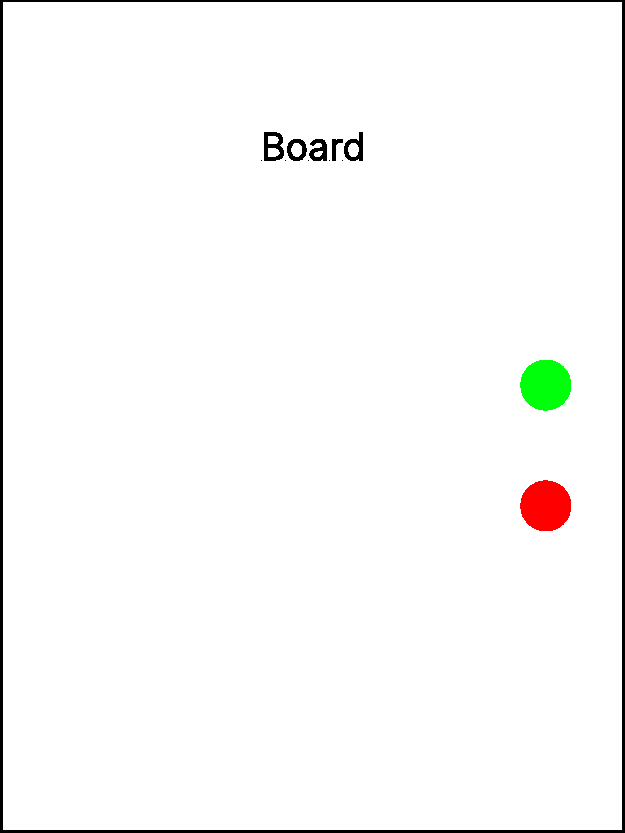
\includegraphics[width=0.4\textwidth]{LedSoftPorte}
    \caption{Vue Board}
    \label{Vue Board}
\end{figure}

La LED LD5 située sur la Board s'allume en vert afin de signaler le bon fonctionnement de SoftPorte. 
S'il y a eu un démarrage incorrect la LED ne s'allume pas.

La LED LD6 située sur la Board s'allume en rouge si le visage du Testeur n'est pas reconnu.
Si le visage est reconnu la LED ne s'allume pas. 


\newpage
\subsection{Description des fonctions}
\hypertarget{fcnid}{}

\underline{Identifier un visage}

L'algorithme de la fonction "identifier un visage" est décrit par un diagramme d'activité UML en figure \ref{idVisage}.

\begin{figure} [H]
    \centering
    \includegraphics[scale=0.8]{fonction_identifie_visage}
    \caption{Algorithme de la fonction "Identifier un visage"}
    \label{idVisage}
\end{figure}

L'algorithme de reconnaissance faciale est effectué par le programme Recognize basé sur une libraire de reconnaissance faciale propriétaire appartenant au client. 

Il est convenu que le programme Recognize n'est pas fourni par l'équipe projet au client.
Il appartient au client d'implémenter ce programme pour permettre le bon fonctionnement du système.

\newpage
\setglossarysection{subsection}
\printglossary[title=Dictionnaire du domaine] \label{dictionnaireDomaine}
\glsaddallunused

%-----------------------------------------
%      Partie IV
%-----------------------------------------
\input{sections/4.Signatures.tex}


\newpage
\listoffigures \label{TableOfFigure} % Affiche la table des figures

%\printbibliography[heading=bibnumbered, label=bibliography] % Affiche les références/bibliographie
%\nocite{*} % Afficher toutes les références (même celles non utilisées)

\end{document}